\documentclass[12pt, a4paper]{extarticle}
\usepackage{amsfonts}
\usepackage[T2A]{fontenc}
\usepackage[utf8]{inputenc}
%\usepackage{mathtext}  
\usepackage{amsmath, amsfonts, amssymb}
\usepackage[russian]{babel}
\usepackage[body={17.5cm, 23.5cm},left=3cm, top=2cm, right=2cm]{geometry}
\usepackage{graphicx}
\usepackage{blindtext}
\usepackage{fancyhdr}
\usepackage{graphicx}
\usepackage{ragged2e}
\usepackage{epigraph}
\usepackage{misccorr}  
\usepackage{indentfirst} 
\usepackage{amsmath}
\usepackage{tabularx} 

\usepackage{fancyhdr} 
\usepackage{color}

%\parindent{1.25cm} 
\graphicspath{images/}
\setcounter{tocdepth}{6}
\newcommand{\eps}{\varepsilon}
\newcommand{\re}{\operatorname{Re}}
\newcommand{\im}{\operatorname{Im}}
\DeclareMathOperator{\sgn}{sgn}
\renewcommand{\labelitemi}{$-$}
\renewenvironment{itemize}[1][{---\hfil}]{\begin{list}{#1}{\topsep=0pt\parsep=0pt plus 1pt\itemsep=\parsep\leftmargin=0pt \itemindent=\parindent}\addtolength{\itemindent}{\labelwidth}}{\end{list}}

\numberwithin{equation}{section} 

\newtheorem{attachment}{\hspace{12cm}  Приложение}
\renewcommand{\theattachment}{\Alph{attachment}}
%\renewcommand{\newtheorem}{\Alph{attachment}}
%\newtheorem{Conjecture}{Conjecture}[section]

\usepackage{tocloft}
\renewcommand{\cftsecleader}{\cftdotfill{\cftdotsep}}

\begin{document}
\thispagestyle{empty} 
\medskip 

\begin{center} 
	\textbf{МИНОБРНАУКИ РОССИИ\\ 
		\vspace{0.5cm} 
		Федеральное государственное бюджетное образовательное\\ 
		учреждение высшего образования\\ 
		«Ярославский государственный университет им. П.Г. Демидова»}\\ 
	\vspace{0.5cm} 
	{Кафедра математического моделирования}\\ 
	\vspace{1.5cm} 
	
\end{center}
\begin{flushright} 
	Сдано на кафедру\\
	« 
	\underline{\phantom{aaa}} 
	» 
	\underline{\phantom{aaaaaaaaaaaaa}} 2018 г.\\ 
	Заведующий кафедрой\\
	\underline{\phantom{aaa}д. ф.-м. н., профессор\phantom{aaa}}\\ 
	\vspace{0.1cm} 
	\underline{\phantom{aaaaaaaaaaaaa}} С.А. Кащенко
\end{flushright}
\vspace{3cm} 
\begin{center} 
	Выпускная квалификационная работа\\ 
	\vspace{0.5cm} 
	\textbf{Компьютерное моделирование движения физических объектов}\\ 
	\small{(Направление подготовки бакалавров 01.03.02 Прикладная математика и информатика)}
	\vspace{3cm} 
\end{center} 

\begin{flushright} 
	Научный руководитель\\ 
	\underline{\phantom{aaa}канд. ф-м. н., доцент\phantom{aaa}}\\ 
	\vspace{0.1cm} 
	\underline{\phantom{aaaaaaaaaaaaa}} И.С. Кащенко\\ 
	« 
	\underline{\phantom{aaa}} 
	» 
	\underline{\phantom{aaaaaaaaaaaaa}} 2018 г.\\ 
	\vspace{0.5cm} 
	Студент группы \underline{\phantom{a}ПМИ-42БО\phantom{a}}\\ 
	\vspace{0.1cm} 
	\underline{\phantom{aaaaaaaaaaaaa}} М.А. Погребняк\\ 
	« 
	\underline{\phantom{aaa}} 
	» 
	\underline{\phantom{aaaaaaaaaaaaaa}}2018 г.\\ 
	\vspace{1cm} 
\end{flushright} 
\begin{center} 
	Ярославль 2018 г.
	\vspace{-1cm}  
\end{center} 


\justify 
\setlength{\parindent}{1.25cm} 
\newpage 
\thispagestyle{empty} 
\setcounter{page}{2} 
\section*{Реферат}
\vspace{\baselineskip}	

\newpage

\setcounter{page}{2}

%\thispagestyle{empty} 
\tableofcontents 
\newpage 

\section*{Введение}
\addcontentsline{toc}{section}{Введение}
\epigraph{\textit{цитата}}
{-- автор}
В современном мире, где технологии и прогресс с огромной скоростью шагают вперёд, трудно представить, как человек смог бы обходится без мощного инструмента познания окружающей действительности под названием «математическое моделирование». С момента появления человека на земле математическое моделирование стало неотъемлемой частью его жизни. Необходимость в исследовании математических моделей прежде всего влияет на саму жизнь человека. Оно возникает, когда сами объекты или явления недоступны для изучения ввиду опасности, которую они представляют, удалены во времени и в пространстве или исследования связанны с большими материальными потерями и непредвиденными последствиями. Так или иначе математическое моделирование имеет огромную важность в жизни человека и никогда не потеряет свою актуальность.

В настоящее время, в связи с развитием компьютерной техники и постоянным совершенствованием программного обеспечения, математическое моделирование развивается быстрыми темпами. Возрастающие потребности в различных сферах общества, например, разработка и управление техническими устройствами, анализ экономических и социальных процессов, способствуют этому. Все естественные и общественные науки, использующие математический аппарат, по сути занимаются математическим моделированием: заменяют реальный объект его моделью, а затем его изучают. Результаты таких исследований очень содержательны и применимы в повседневной жизни, так как сама идея математического моделирования заключается в замещении изучаемого объекта его аналогом, отражающим в математической форме важнейшие его свойства. Математическая модель выражает существенные черты объекта или процесса языком уравнений и других математических средств. 

Метод математического моделирования занимает одно из ведущих мест в исследованиях сложных явлений и процессов, так как позволяет количественно и качественно описать наиболее существенные связи между переменными в системе и применить достаточно развитый математический аппарат и программные средства для анализа явлений, а также для их прогнозирования и управления этими процессами. 

Математическое моделирование очень часто встречается в физике, ведь не зря математику называют языком физики. Эти науки всегда тесно связаны и взаимно обогащают друг друга идеями и методами. Хотя физика и считается наукой о природе, изучающая простейшие и вместе с тем наиболее общие свойства материального мира, но она базируется на моделях объектов материального мира. Поэтому метод математического моделирования изначально зародился в физике, точнее, в математической физике, а затем постепенно начал проникать и в другие науки, где со временем стал очень востребован. Раньше из обширного математического аппарата физики применяли в основном аналитические и полуаналитические методы и приёмы Сейчас все чаще обращаются к математическому моделированию, когда исследуемый физический процесс описывается некоторой математической моделью, представляющей собой систему дифференциальных или интегро-дифференциальных уравнений математической физики. Изучая какие-либо физические явления, исследователь прежде всего создаёт его математическую идеализацию или, другими словами, математическую модель, то есть, пренебрегая второстепенными характеристиками явления, он записывает основные законы, управляющие этим явлением, в математической форме и очень часто эти законы выражаются в виде дифференциальных уравнений. Для составления математической модели в виде дифференциальных уравнений нужно, как правило, знать только локальные связи и не нужна информация обо всем физическом явлении в целом.

Современные компьютерные технологии позволили подойти к решению проблемы математического моделирования транспортных потоков. Основы математического моделирования, закономерностей дорожного движения были заложены в 1912 году русским учёным, профессором Г.Д. Дубелиром. В своей книге «Городские улицы и мостовые» он положил начало развитию такой отрасли как моделирование транспортных потоков. За прошедший век непрерывных исследований выработалось много хороших моделей, которые помогают сегодня строить качественные и быстрые дороги и регулировать транспортные потоки. Но проблема транспортных потоков никуда не уходит, а на оборот только возрастает в связи с увеличением численности людей на земле, строительством и расширением городов и сообщений между ними и как следствие развитием и модернизацией транспорта.  Транспорт— одна из ключевых систем городского организма, которую по важности уместно сравнить с кровоснабжением. Именно транспорт позволяет городу в полной мере выполнять связующую, коммуникационную и обеспечивающую функции. Тема транспорта касается практически каждого городского жителя, и тем важнее становятся усилия по систематизации управления дорожным движением на транспортной сети городов, ведь без грамотно проработанной транспортной модели, управлять городскими потоками практически, невозможно. Например, в определённом месте городской магистрали систематически возникают автомобильные пробки. Если модель транспортной системы отсутствует, высока вероятность принятия ошибочного решения, результатом которого станет перенос пробки на новое место или создание новых автомобильных пробок. Создавая подобные модели, можно планировать транспортные системы современных городов. Изменения в одной части такой системы приводят к появлению изменений в других ее частях. Насколько увеличится автомобильный поток, если сделать дорогу более широкой? Почему автомобильная пробка регулярно образуется на конкретном перекрёстке? Какой потенциал создаст развитие системы городского общественного транспорта для изменения застройки в черте города? Что случится, если внести изменения в режим работы определённого светофора? Ответить на все эти, а также многие другие вопросы позволяет моделирование транспортной системы. Одна из наиболее трудных проблем, стоящих перед исследователем
организации движения — это превращение реальной дорожно-транспортной обстановки, включающей водителей, автомобили, устройства регулирования движения и дорогу, в набор математических символов и зависимостей, воспроизводящих их поведение. Именно тут математическое моделирование является основой, которая позволяет рассматривать подобные взаимодействия в целом. Решение задач моделирования транспортных потоков и внедрение этих технологий позволяет значительно улучшить ситуацию на проезжей части дороги, снизить тенденцию к образованию транспортных пробок, перегрузке или недогрузке отдельных линий и узлов транспортной сети, снижению уровня аварийности, а также помогает решать и экологические проблемы.

\newpage

\section{Постановка задачи} 
  

\newpage
\section{}
Научное исследование транспортных потоков началось ещё в 1910-х годах прошлого века с применением различных теорий и методов. Было создано множество моделей для описания потоков движения: модели, основанные на теории клеточных автоматов, газокинетические модели, гидродинамические модели и другие. Но основным теоретическим подходом исследования движения транспортных потоков является  модель движения транспортных средств друг за другом.

Под \textbf{Транспортным потоком} будем понимать {\it количество единиц транспортных средств одного вида транспорта, проследовавших определённый участок пути в течение установленного промежутка времени} \cite{TrafficFlow}. В качестве транспортного средства рассмотрим автомобиль и будем называть его \textbf{лидером}, если за ним есть другой автомобиль, или \textbf{преследователем}, если перед ним есть другой автомобиль. Причём один и тот же автомобиль может являться одновременно и преследователем для впереди идущего, и лидером для позади идущего рис. \ref{car_following}. 

\begin{figure}[h!]  
	\begin{center}
		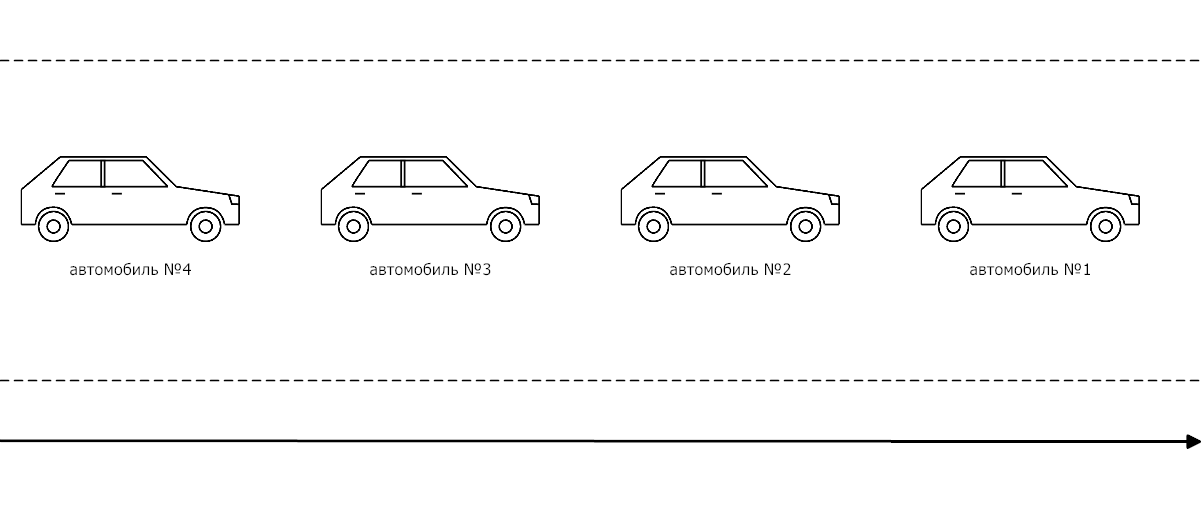
\includegraphics[keepaspectratio,width=160mm,height=70mm]{Images/car_following.png}
	\end{center}
	\caption{Следующие друг за другом автомобили.}
	\label{car_following}
\end{figure}

Рассмотрим парадигму автомобиля, которая основана на очень простом правиле и уже довольно давно известна в литературе, так как автомобили следуют друг за другом, преследователь всегда пытается максимизировать свою скорость с двумя ограничениями: ограничением ускорения и ограничением безопасности. Впервые данная парадигма была высказана ещё в 1975 \cite{GippsModel} и математически выглядит следующим образом:

\begin{equation} \label{following_paradigm}
v_f(t) = \min(v_f^d(t), v_f^s(t))
\end{equation}
где $v_f(t)$ - скорость преследователя в момент времени $t$, $v_f^d(t)$ - максимальная возможная скорость с \textbf{ограничением ускорения} (demand speed), $v_f^s(t)$ - максимальная возможная скорость с \textbf{ограничением безопасности} (supply speed).

Под ограничение ускорения стоит понимать физических ограничения скорости и ускорения транспортного средства, а также комфортные условия для водителя. Оно описывает траекторию транспортного средства, которое свободно разгоняется до максимальной желаемой скорости при отсутствии впереди идущих транспортных средств. Это не всегда постоянное значение: например, оно может зависеть от скорости автомобиля (см. \ref{following_paradigm}). Ограничение безопасности - это то, как траектория транспортного средства зависит от впереди транспортного средства (лидера).


\section{Модель следования за лидером без остановки}

Рассмотрим дифференциальное уравнение, которое описывает ускорение транспортного средства \eqref{equation_for_acceleration}.

\begin{equation} \label{equation_for_acceleration}
\ddot{x}(t) = d (\dot{x}(t-\tau)-\dot{x}(t)),
\end{equation}
где $d$ - мощность двигателя, а $\tau$ - время реакции водителя.

Уравнение \eqref{equation_for_acceleration} зависит от скорости движения двух соседних автомобилей, то есть водитель автомобиля должен смотреть только на впереди идущий автомобиль. Конечно, в реальной жизни, водитель следит за движем большего количества транспортных средств вокруг него, например справа и слева, но при движении по прямой без перестроений их влияние минимально.

Проинтегрировав уравнение \eqref{equation_for_acceleration} получаем уравнение  \eqref{equation_for_speed}

\begin{equation} \label{equation_for_speed}
\dot{x}(t) = d(x(t-\tau) - x(t) - \lambda),
\end{equation}
где $\lambda$ - безопасное расстояние между автомобилями.

Уравнение \eqref{equation_for_speed} не удобно для анализа, поэтому запишем его в виде разностной системы уравнений:

\begin{equation} \label{equation_without_stopping}
\begin{cases}
\begin{split}
&\dot{x}_1(t) = d (v_{\max} t - x_1(t) - \lambda), \\ 
&\qquad x_1(0) = 0, \\
&\dot{x}_2(t) = d (x_1(t-\tau)-x_2(t) - \lambda), \\
&\qquad x_2(t) = -\lambda \quad t \in [-\tau, 0], \\
&\dot{x}_3(t) = d (x_2(t-\tau)-x_3(t) - \lambda), \\
&\qquad x_3(t) = -2\lambda \quad t \in [-2\tau, 0], \\
&\ldots \\
&\dot{x}_n(t) = d ({x}_{n-1}(t-\tau)-x_n(t) - \lambda), \\
&\qquad x_3(t) = -(n-1)\lambda \quad t \in [-(n-1)\tau, 0], \\
&\ldots \\
\end{split}
\end{cases}
\end{equation}

Обозначения, использующиеся в системе \eqref{equation_without_stopping}, приведены в таблице \ref{parameters}:

\begin{table}[h]
	\caption{Физическое значение параметров}
	\label{parameters}
	\begin{center}
		\begin{tabularx}{\textwidth}{p{0.15\linewidth}p{0.85\linewidth}}
			
			\hline
			\rule{0cm}{0,5cm}
			Параметр &  Физическое значение \\ 
			[3pt]\hline
			-- & -- \\
			\hline
		\end{tabularx}
	\end{center}
\end{table}


\begin{figure}[h!]
	\begin{center}
		\begin{minipage}[h!]{0.48\linewidth}
			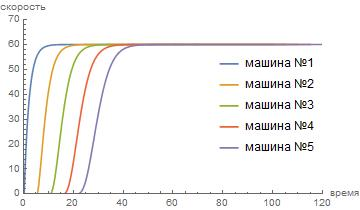
\includegraphics[width=1\linewidth,height=0.2\textheight]{Images/speed_without_stop_d=0,5.jpg}
			\label{fall_3d}
		\end{minipage}
		\hfill 
		\begin{minipage}[h!]{0.48\linewidth}
			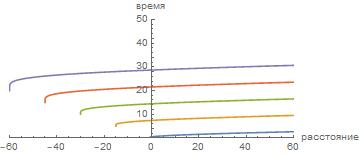
\includegraphics[width=1\linewidth,height=0.2\textheight]{Images/distance_without_stop_d=0,5.jpg}
			\label{contact_3d}
		\end{minipage}
	\caption{Касание плоскости одной вершиной.}
	\end{center}
\end{figure}


\section{Модель следования за лидером с остановкой}
 
\section{Реализация} 
 

\newpage
\section*{Заключение}
\addcontentsline{toc}{section}{Заключение}

\newpage

\begin{thebibliography}{**}
	\bibitem{TrafficFlow}
	https://spravochnick.ru/logistika/logisticheskie\_potoki/transportnyy\_potok/
	\bibitem{GippsModel}
	Wilson R. E. Gipps’ Model of Highway Traffic. 2002.
	\bibitem{Polygon}
	Выгодский М.Я. Справочник по элементарной математике. 2001.
 	\bibitem{Runge_Kutta}
	 Бахвалов Н.С.  Численные методы. 1975.  
	\bibitem{Refactoring}
	Мартин Ф. Рефакторинг. Улучшение существующего кода. 2008.
\end{thebibliography}

\end{document}